\section{A Diversion Scenario: Highly Enriched Uranium}
\label{s_results}
As a part of the \gls{CVT}\footnote{http://cvt.engin.umich.edu/}, \Cyclus is being used to incorporate social-behavioral modeling into simulations of \gls{HEU} diversion from a declared fuel cycle.  In the simplest implementation, material is diverted from the enrichment facility.  Figure \ref{fig:heu_layout} illustrates a toy model of this portion of the fuel cycle. A facility such as a mine supplies natural uranium (0.7\% $^{235}$U) to an enrichment facility.  The enrichment facility in turn receives requests for  \gls{LEU} (4\% $^{235}$U) from a declared light-water reactor (ignoring the fuel fabrication facility for simplicity).  The enrichment facility also receives requests for 90\% enriched \gls{HEU} from an undeclared actor seeking to build a nuclear weapon. Material flow, or throughput, out of each facility is calculated once each month for a total of 100 months.  This framework allows us to pose the following question: If an inspector only has access to the inventory records for the \gls{LEU} that arrives at the declared reactor, can diversion of material be detected?

\begin{figure}%[htbp!]
\begin{center}
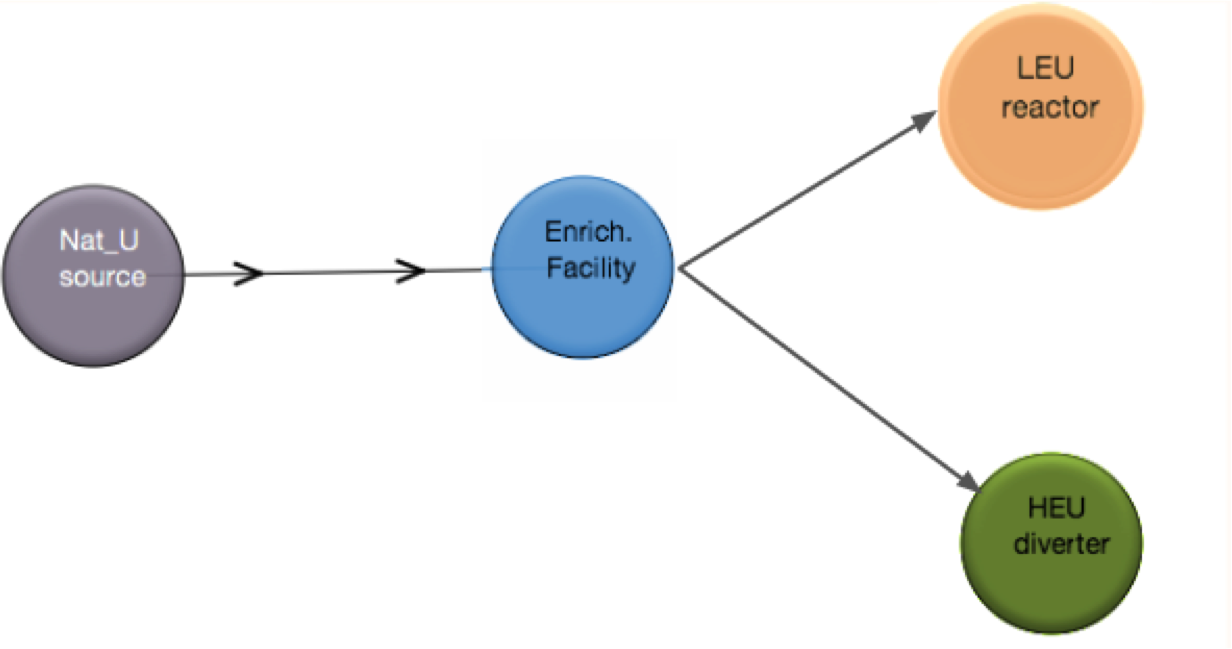
\includegraphics[natwidth=162bp,natheight=227bp, scale=0.7]{./figs/heu_cyclist_layout.png}
\end{center}
\caption{Agent layout and material flow for a toy model of \gls{HEU} diversion from a declared fuel cycle at the enrichment facility.}
\label{fig:heu_layout}
\end{figure}

To make the scenario more realistic, three conditions are applied to the simulation:
\begin{itemize}
\item{The enrichment facility is nominally operating near its maximum \gls{SWU} limit}
\item{The demand for \gls{LEU} material has a time-varying amplitude with a Gaussian distribution}
\item{The enrichment facility will always prioritize fulfilling requests for \gls{HEU}}
\end{itemize}
The \gls{SWU} limit, a metric that incorporates power-consumption and maximum processing throughput, constrains the simulation so that if the enrichment facility chooses to produce \gls{HEU} then its \gls{LEU} output will necessarily decrease.  If the \gls{LEU} demand were constant then there would be a clear signature of diversion when \gls{HEU} was produced and the simulation would be trivial.  A time-variation in \gls{LEU} demand is more representative of real-life, where a single enrichment facility provides fuel to many reactors, which may operate on different reloading schedules. Variations in demand can also be caused by unanticipated reactor shutdowns, delays in receiving raw material, maintenance and repairs, etc.  While these events are somewhat mitigated in real operations by the use of long-term contracts and material reserves, a small variation in nominal \gls{LEU} demand is a reasonable assumption.

% Simulation parameters in RS_3sink.xml at
%/Users/mbmcgarry/git/data_analysis/data/v1.2/random_sink/
\begin{table}
\centering
\begin{tabular}{|c|c|c|}
\hline
\textbf{General}    & Duration (months)      & 100  \\
\textbf{Simulation} & Natural U \% $^{235}U$ & 0.7  \\
                    & LEU \% $^{235}U$    & 4.0  \\
                    & HEU \% $^{235}U$    & 90.0 \\
\hline
\textbf{Enrichment} & SWU Capacity (kg-SWU/month) & 180  \\
\textbf{Facility}   & Tails Assay (\% $^{235}U$)   & 0.3  \\
\hline
\textbf{LEU Demand} & Mean Qty (kg)       & 33.0  \\
                    & $\sigma$ (kg)       & 0.5  \\
\hline
\textbf{HEU Demand} & Qty (kg)            & 0.03  \\
                    & Avg Occur. (months) & 1/5 \\ 
\hline
\end{tabular}
\caption{Simulation parameters for \gls{HEU} diversion scenario.}
\label{tab:sim_params}
\end{table}


Several behavioral models have been explored to parameterize the behavior of the illicit actor who is requesting \gls{HEU}.   In the scenario presented here, the actor asks for the same quantity of material in each request, but the requests do not have a constant frequency. Rather they are modeled as occurring `randomly' with a Gaussian distribution that defines their average rate of occurrence.  Other models that have been examined include diversion at regular intervals, as well as independent engagement decision-making for both the illicit actor and the enrichment facility.  Table \ref{tab:sim_params} lists the parameters used for the simulation, where \gls{HEU} is diverted using the `random' model with an average occurrence rate of once per 5 months.  Figure \ref{fig:heu_demand} shows the \gls{HEU} demand from the illicit actor as a function of time.  Figure \ref{fig:leu_produced} illustrates the impact of this illicit material diversion on overall \gls{LEU} production.  The orange trace represents the amount of \gls{LEU} material that would have been produced by the enrichment facility at each timestep if there had been no material diversion for \gls{HEU} production.  The blue trace represents the amount of \gls{LEU} that was actually produced and shipped to the declared reactor during the diversion scenario.


% Figures made with ~/git/data_analysis/fourier_analysis.ipynb, and saved in
% /Users/mbmcgarry/git/data_analysis/data/v1.2/random_sink/png
\begin{figure}
\begin{center}
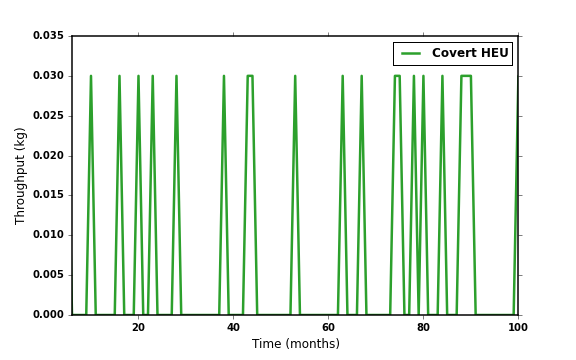
\includegraphics[natwidth=162bp,natheight=227bp, scale=0.7]{./figs/HEU_R5.png}
\end{center}
\caption{An illicit actor request \gls{HEU} from the enrichment facility at random timesteps with an average occurrence rate of 1 out of every 5 months \TODO{Update label 'diverted HEU'}}
\label{fig:heu_demand}
\end{figure}

\begin{figure}
\begin{center}
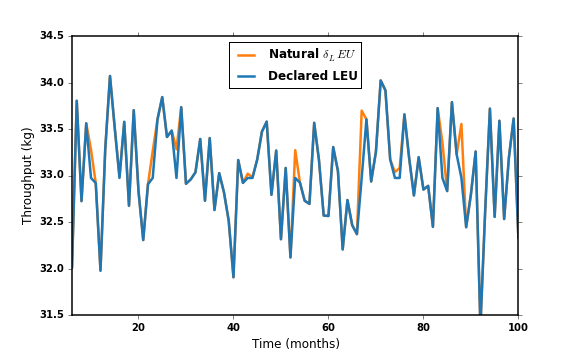
\includegraphics[natwidth=162bp,natheight=227bp, scale=0.7]{./figs/nat_delta_R5.png}
\end{center}
\caption{Expected variation of \gls{LEU} demand in the absence of diversion is shown in orange, while the \gls{LEU} actually produced in the diversion scenario is shown in blue. The amplitude of the diverted material was chosen to displace the signal with one standard deviation of the expected variation. \TODO{Update labels: Expected and Declared LEU}}
\label{fig:leu_produced}
\end{figure}


\begin{figure}
\begin{center}
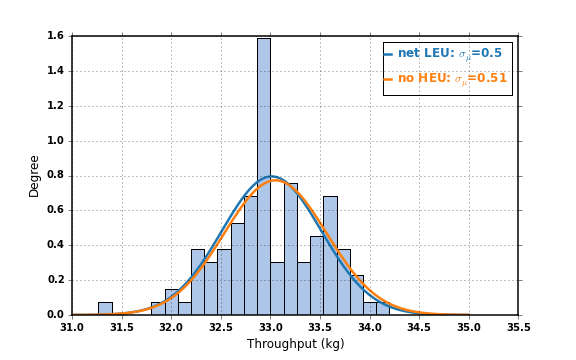
\includegraphics[natwidth=162bp,natheight=227bp, scale=0.7]{./figs/netLEU_hist_R5_new.png}
\end{center}
\caption{The expected variation of \gls{LEU} demand in the absence of diversion is shown in orange, while the \gls{LEU} actually produced in the diversion scenario is shown in blue.  A shift of the fitted peak indicates that material is being diverted.\TODO{update labels: Declared, Expected}}
\label{fig:leu_histogram}
\end{figure}

If the inspector has access to only the blue time-series data, is it possible to identify whether or not material is being diverted from the system?  A naive approach is to look at the distribution of the time-series data.  Figure \ref{fig:leu_histogram} is a histogram of the declared \gls{LEU} signal.  The blue trace is a Gaussian fit to the declared data, while the orange trace (``expected'') is a Gaussian fit to the hypothetical variation in the \gls{LEU} signal if there were no diversion.  In this example, an inspector would need a sufficiently well-sampled dataset for the facility during a time when there was no diversion to characterize the expected distribution in order to draw conclusions about whether or not material diversion is occurring. An ongoing collaboration with researchers at the Michigan Institute for Data Science\footnote{http://midas.umich.edu/} seeks to apply innovative anomaly detection techniques to these simulations to investigate detection limits for scenarios with sparse data sets or low signal-to-noise ratios.





  
